\documentclass[tikz,border=3mm]{standalone}
\usetikzlibrary{matrix}
\begin{document}
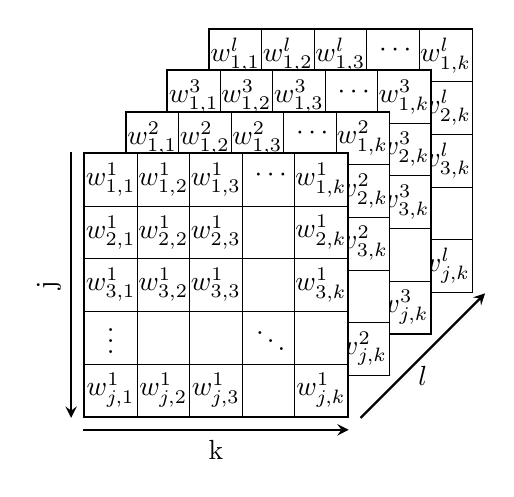
\begin{tikzpicture}[auto matrix/.style={matrix of nodes,
  draw,thick,inner sep=0pt,
  nodes in empty cells,column sep=-0.2pt,row sep=-0.2pt,
  cells={nodes={minimum width=1.9em,minimum height=1.9em,
   draw,very thin,anchor=center,fill=white,
   execute at begin node={%
   $\vphantom{x_|}\ifnum\the\pgfmatrixcurrentrow<4
     \ifnum\the\pgfmatrixcurrentcolumn<4
      {w}^{#1}_{\the\pgfmatrixcurrentrow, \the\pgfmatrixcurrentcolumn}
     \else
      \ifnum\the\pgfmatrixcurrentcolumn=5
       {w}^{#1}_{\the\pgfmatrixcurrentrow, k}
      \fi
     \fi
    \else
     \ifnum\the\pgfmatrixcurrentrow=5
      \ifnum\the\pgfmatrixcurrentcolumn<4
       {w}^{#1}_{j, \the\pgfmatrixcurrentcolumn}
      \else
       \ifnum\the\pgfmatrixcurrentcolumn=5
        {w}^{#1}_{j, k}
       \fi
      \fi
     \fi
    \fi
    \ifnum\the\pgfmatrixcurrentrow\the\pgfmatrixcurrentcolumn=14
     \cdots
    \fi
    \ifnum\the\pgfmatrixcurrentrow\the\pgfmatrixcurrentcolumn=41
     \vdots
    \fi
    \ifnum\the\pgfmatrixcurrentrow\the\pgfmatrixcurrentcolumn=44
     \ddots
    \fi$
    }
  }}}]
  \matrix[auto matrix=l,xshift=4.5em,yshift=4.5em](matz){
  & & & & \\
  & & & & \\
  & & & & \\
  & & & & \\
  & & & & \\
 };
 \matrix[auto matrix=3, xshift=3em,yshift=3em](mate){
  & & & & \\
  & & & & \\
  & & & & \\
  & & & & \\
  & & & & \\
 };
 \matrix[auto matrix=2,xshift=1.5em,yshift=1.5em](maty){
  & & & & \\
  & & & & \\
  & & & & \\
  & & & & \\
  & & & & \\
 };
 \matrix[auto matrix=1](matx){
  & & & & \\
  & & & & \\
  & & & & \\
  & & & & \\
  & & & & \\
 };
 \draw[thick,-stealth] ([xshift=1ex]matx.south east) -- ([xshift=1ex]matz.south east)
  node[midway,below] {$l$};
 \draw[thick,-stealth] ([yshift=-1ex]matx.south west) --
  ([yshift=-1ex]matx.south east) node[midway,below] {k};
 \draw[thick,-stealth] ([xshift=-1ex]matx.north west)
   -- ([xshift=-1ex]matx.south west) node[midway,above,rotate=90] {j};
\end{tikzpicture}
\end{document}